\clearpage
\begin{appendices}
\section{Optimization Process Details}

\subsection{Hessian Scaling Procedure}\label{sec:appendix-scaling}
First the unscaled optimization is run for a small number (8) of iterations to obtain a realistic Hessian $H$.
Then a scale vector $\textbf{s}$ with elements $s_i$ is calculated from the diagonal Hessian entries, as recommended in section 8.3 of reference text \cite{papalambros_principles_2017}:
\begin{equation}
    s_i = \frac{1}{\sqrt{H_{ii}}}
\end{equation}
A new scaled optimization problem is solved using the scaled design variables $\textbf{x}_s$:
\begin{equation}
\begin{aligned}
    \text{min}~~& \textbf{J}(\textbf{x}_s \odot \textbf{s},~\textbf{p}) \\
    \text{by varying}~~&\textbf{x}_s= \textbf{x} \varoslash \textbf{s}\\
    \text{subject to}~~ &\textbf{x}_{LB}\varoslash \textbf{s} \leq \textbf{x}_s \leq \textbf{x}_{UB} \varoslash \textbf{s}\\
    &\textbf{g}_{NL}(\textbf{x}_s\odot\textbf{s},~\textbf{p}) \geq 0\\
    & (A_{ineq} \odot \textbf{s}^T)\textbf{x}_s \leq b_{ineq}
\label{standard}
\end{aligned}
\end{equation}
where $\odot$ indicates element-wise matrix multiplication and $\varoslash$ element-wise matrix division.

\subsection{Hyper-parameters}\label{sec:appendix-extra-param}
Table~\ref{tab:hyperparams} documents the hyper-parameters used to control convergence and other numerical aspects of the simulation and optimization.
\begin{table}
    \centering
    \begin{tabular}{|l|c|c|c|} \hline 
          &Variable&  Value& Unit\\ \hline 
          Simulation&$X_{tol}$&  0.01 & m \\ \hline 
          &$\angle X_{tol}$& 3 & degrees\\ \hline 
          &Maximum drag iterations& 100 & -\\ \hline 
          &$N_{harmonics}$& 10 & - \\ \hline
          &$b_{max}$ & 700.5 & - \\ \hline
          SQP Optimization&Constraint tolerance& 1e-5 & - \\ \hline
          &Iterations before Hessian scaling& 8 & - \\ \hline
  &Maximum iterations after Hessian scaling& 150&-\\\hline
  &Maximum function evaluations& 2000&-\\\hline
 Multi-objective optimization& Number of epsilon-constraint seeds& 8&-\\\hline
 & Minimum poll fraction& 1&\\\hline
 & Pareto set change tolerance& 1.6e-8&\\\hline
 & Maximum pattern search iterations& 100&\\\hline
    \end{tabular}
    \caption{Hyper-parameters used to control numerics}
    \label{tab:hyperparams}
\end{table}

\clearpage
\section{Supplementary Results}
\label{sec:appendix-supplemental-results}

\subsection{Single Objective Optimization Results}
\figureautorefname~\ref{fig:gradient} depicts the normalized gradient.
A value of zero is expected if the design variable is not involved in an active constraint.
Notably, all values are nonzero, except for $h_{fs,clear}$, which is the only design variable not involved in any active constraint.
Nonzero values convey the amount that the objective would improve if the design variable changed, although changing this design variable would violate the active constraint(s) that the design variable is involved in.

\begin{figure}
\centering
\includegraphics[width=\linewidth]{example-image-a}
\caption{Normalized gradient at optimal point}\label{fig:gradient}
\end{figure}

\figureautorefname~\ref{fig:single-objective-convergence} shows the convergence of the single objective optimization (LCOE minimization) using the nominal RM3 design as a starting point.
\begin{figure}
\centering
\includegraphics[width=\linewidth]{\matlabFilepath{44}}
\caption{Single objective convergence plots}\label{fig:single-objective-convergence}
\end{figure}

Figure~\ref{fig:multistart-parallel-axis} shows the effect of starting point $x_0$ (leftmost column in each subplot) on the optimal design value $x^*$ (middle two columns) and optimal objective value $J^*$ (rightmost two columns).
The meaning of $x$ in each subplot is indicated by the subplot title.
The two starting points that achieve global optima, denoted in green and orange, both have low inital values of $T_{f,2}$ and medium initial values of $t_{f,b}$.
The value of the optimal draft, $T_{f,2}^*$, is likewise lowest at the global minima. 
On the other hand, the optimal float thickness, $t_{f,b}^*$, both depends less on and differs more from the initial value for float thickness.
This suggests that it is primarily the initial value of the draft $T_{f,2}$, rather than the initial float thickness $t_{f,b}$, that is important for arriving at the global optimum.
Figure~\ref{fig:multistart-parallel-axis} also sheds light on the convexity of the search space: local minima are common for all design variables except $T_{f,2}$ and $t_{f,b}$, which usually converge to the same optimal $x^*$ value regardless of the starting point $x_0$.
Surprisingly, the optimal values take on many different continuous values, as opposed to converging to several discrete values as might be expected from distinct local optima in a multimodal problem.
\hl{This requires further investigation to explain and will be done during re-scrutineering.}

\begin{landscape}
\begingroup
\centering

\begin{figure}
\centering
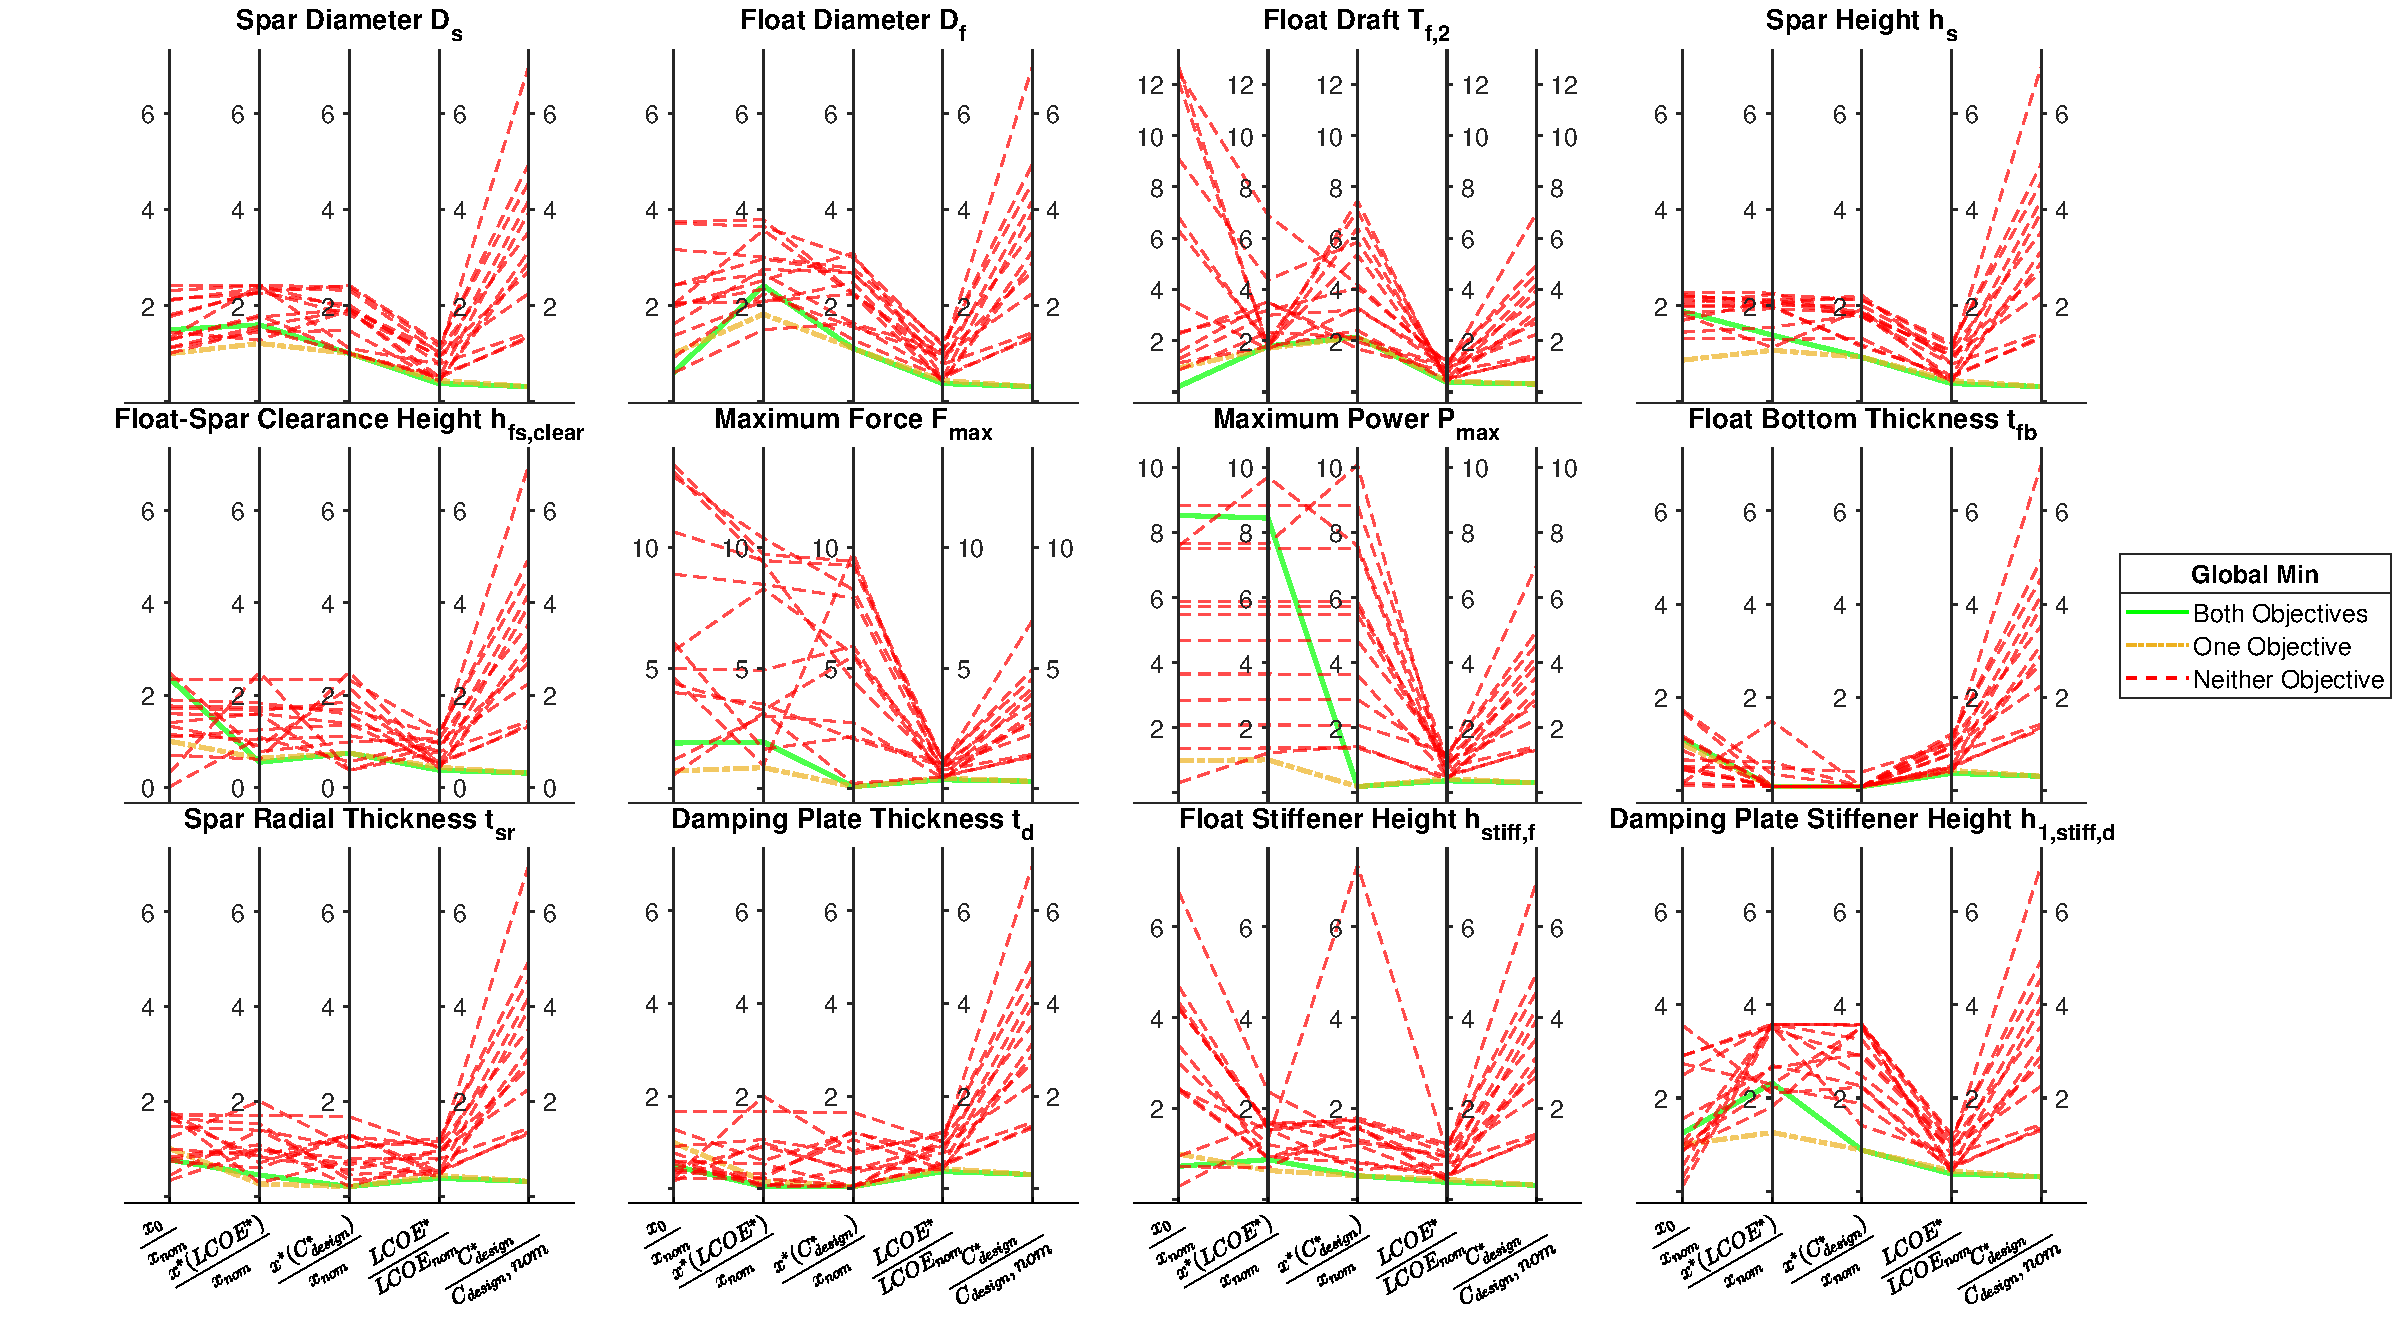
\includegraphics[width=1.2\linewidth]{figs/multistart_parallel_axis.pdf}
\caption{Parallel axis plot for effect of starting point on convergence}\label{fig:multistart-parallel-axis}
\fillandplacepagenumber
\end{figure}

\endgroup
\end{landscape}

\subsection{Local Sensitivities}\label{sec:appendix-sensitivties}
Figure~\ref{fig:param-sens-local-global-J-star}, \ref{fig:param-sens-local-x-star}, and \ref{fig:param-sens-global-x-star} depict the local sensitivities of the optimal objective and optimal design variables, respectively, to parameters. 
\begin{figure}
\includegraphics[width=\linewidth]{\matlabFilepath{16_a}}
\caption{Local parameter sensitivity analysis to optimal objective $J^*$}
\label{fig:param-sens-local-global-J-star}
\end{figure}

\figureautorefname~\ref{fig:param-sens-local-global-J-star} compares four ways of computing the objective total derivative local sensitivity, $\frac{dJ^*}{dp}$.
The first and simplest method uses only the partial derivative, $\frac{dJ^*}{dp}\approx \frac{\partial J}{\partial p}$.
This partial derivative is found via finite difference around the optimal point and does not attempt to take into account the effect of the parameter change on the optimal design $x^*$.
The second method, suggested in \cite{martins_engineering_2022}, uses a linear model to account for the change in $x^*$ due to parameter-dependent constraints.
The change in $x^*$ is not calculated directly and is instead incorporated through the Lagrange multipliers $\lambda$:
\begin{equation}
\frac{dJ^*}{dp} \approx \frac{\partial J}{\partial p} -  \lambda^T \frac{\partial g}{\partial p}
\end{equation}
The third method, proposed in \cite{sobieszczanski-sobieski_sensitivity_1982}, uses a quadratic model that not only takes into account the change of $x^*$ through the parameter-dependent constraints, but also the change of $x^*$ due to the second-order curvature of the objective.
This method involves setting up a simple linear system for each parameter $p_i$ and solving it for the sensitivity vector $\vec{x}_{sens}$:
\begin{equation}
    A_{sens} \vec{x}_{sens}(p_i) = \vec{b}_{sens}(p_i)
\end{equation}
The forms of the parameter-agnostic $A_{sens}$ matrix and the parameter-specific $b_{sens}$ vector are given in \cite{sobieszczanski-sobieski_sensitivity_1982} and not repeated here.
They are computed from solver outputs like the Lagrange multipliers $\vec{\lambda}$, Hessian $\mathbf{H}$, and gradient $\vec{\nabla} J$, as well as other derivatives %\hl{(specify which)} 
obtained here via finite difference simulation evaluations %\hl{(specify how many)} 
without re-optimizing.
The sensitivity vector $\vec{x}_{sens}$ is then used to solve for a number of quantities of interest including the objective parameter sensitivity $dJ^*/dp$ and the optimal design parameter sensitivity $\partial x^*/\partial p$:%, and the parameter change constraint activity threshold $\Delta p_{ij}$ associated with constraint $g_j$:
\begin{equation}
\begin{aligned}
    \frac{dJ^*}{dp_i} &=  \frac{\partial J}{\partial p_i} + C_{sens}\vec{x}_{sens}(p_i) \\
    \partial x^*/\partial p &=  [I ~0] ~\vec{x}_{sens}(p_i) \\
    %\Delta p_{ij} &= \frac{d_{sens,j}}{\vec{e}_{sens,j}^{~T}\vec{x}_{sens}(p_i)}
\end{aligned}
\end{equation}
where additional sensitivity quantities introduced are matrix $C_{sens}$, scalar $d_{sens,j}$, and vector $\vec{e}_{sens,j}$ assembled from the same inputs as $A_{sens}$ and $b_{sens}$ \cite{sobieszczanski-sobieski_sensitivity_1982}.

%\hl{This formula could be cleaned up by making it vectorized.}

The fourth method requires significantly more computational expense than the first three methods, since rather than using post-optimality derivatives, it repeats the optimization with the changed parameter.
This method is the ``ground truth'' local sensitivity against which the other methods can be compared.
While the first three methods take \gradientSensRuntime~to run, the fourth method takes \reoptimSensRuntime, since \numReoptims~separate optimizations are performed.

While the sensitivities computed with post-optimality derivatives enjoy a significant advantage in computational speed over the re-optimization sensitivity, their accuracy is unfortunately low.
The mean absolute error from quadratic to re-optimization-based normalized sensitivities across all parameters is \hl{XX}\%.
For some parameters such as $t_{f,r}/t_{f,b}$, $\$/N$, and $C_{d,spar}$, a large re-optimization sensitivity exists that the other methods miss entirely, predicting as near-zero.
For some such as \hl{XX}, the values are opposite signs.
This could indicate the presence of discontinuities, strong nonlinearities, or the interference of finite precision effects when computing the partial derivatives.

On the bright side, for the majority (\hl{XX}\%) of parameters, the quadratic sensitivity at least correctly predicts the sign and is only inaccurate in the sensitivity magnitude.
Likewise, the quadratic sensitivity typically outperforms the partial and linear sensitivities in more closely matching the re-optimization-based sensitivity, as would be expected.
For example, this occurs for $h$, $H_{s,struct}$, $FOS_{min}$, $D_{d,tu}$, $FOS_{mult,d}$, $D_d/D_s$, $T_s/D_s$, $T_{f,1}/T_{f,2}$, and $F_{heave,mult}$, but not for $T_{struct}$ or $\eta_{pto}$.
All in all, the quadratic post-optimality sensitivities are useful for rapidly evaluating directional effects without the need to re-optimize, but lack the accuracy required to predict effect magnitudes, which is necessary to screen for parameters with significant effects and appropriately prioritize parameters in order of importance. 

Figures~\ref{fig:param-sens-local-x-star} and \ref{fig:param-sens-global-x-star} depict the normalized local parameter sensitivities of the optimal design.
Even more significant discrepancies are observed than in the objective sensitivities, although both methods agree that the two structural thicknesses $t_{f,b}$ and $t_d$ are insensitive to all parameter changes investigated, likely because they remain at their lower bound.
This reinforces the decision to utilize the re-optimization based sensitivities to draw conclusions despite their higher computational cost.
\begin{figure}
\includegraphics[width=\linewidth]{\matlabFilepath{17_a}}
\caption{Quadratic parameter sensitivity analysis to optimal design $x^*$}
\label{fig:param-sens-local-x-star}
\end{figure}

\begin{figure}
\includegraphics[width=\linewidth]{\matlabFilepath{18_a}}
\caption{Re-optimization parameter sensitivity analysis to optimal design $x^*$}
\label{fig:param-sens-global-x-star}
\end{figure}

Finally, the authors note that while the re-optimization method is valid even when the parameters are far from their nominal values and can be considered a global sensitivity analysis method, it has here only been performed for parameters perturbed in a OAT fashion very close to the nominal and is therefore used as a local sensitivity analysis method.
The global sensitivities of section \ref{sec:sensitivities} only investigate a few select parameters.
Future work could obtain fuller global sensitivities through re-optimization or a variety of other methods such as Sobol variance decomposition or Method of Morris \cite{reed_addressing_2022}.
This would reveal higher order effects like interactions between parameters and dependence of the sensitivity derivative on the parameter value.


\end{appendices}